\documentclass[12pt]{report}

\usepackage[a4paper,width=150mm,top=25mm,bottom=25mm,bindingoffset=6mm]{geometry}
\usepackage[onehalfspacing]{setspace}
\usepackage{ucs}
\usepackage[table,xcdraw]{xcolor}
\definecolor{mColor1}{rgb}{0.9,0.9,0.9}

\usepackage{fancyhdr}
\pagestyle{fancy}
\fancyhead{}
\renewcommand{\chaptermark}[1]{\markboth{#1}{}}
\renewcommand\sectionmark[1]{\markright{\thesection\ #1}}

\fancyhead[LO, RE]{\leftmark}
\fancyhead[LE, RO]{\rightmark}

\usepackage{titlesec, blindtext, color}
\definecolor{gray75}{gray}{0.75}
\usepackage{mathptmx}
\usepackage[utf8]{inputenc}
\usepackage[T1]{fontenc}
\usepackage[ngerman]{babel}

\usepackage{amsmath,amssymb,amstext,amsthm,mathtools}
\usepackage{url}
\usepackage{caption}
%\usepackage[belowskip=-5pt,aboveskip=0pt]{caption}
\usepackage{subcaption}

\usepackage{float}
\usepackage{lscape}
\usepackage{pdfpages}
\usepackage{rotating}
\usepackage{graphicx}
\setlength\parindent{0pt}
\usepackage{hyperref}
\usepackage{acronym}
\usepackage{textcmds}
\usepackage{longtable}
\usepackage[export]{adjustbox}
\usepackage{upgreek}
\usepackage{dsfont}
\usepackage{tensor}
\usepackage{amsbsy}
\usepackage{multirow, hhline, colortbl}
\usepackage[table]{xcolor}


\DeclareMathAlphabet{\mathcal}{OMS}{cmsy}{m}{n}
\SetMathAlphabet{\mathcal}{bold}{OMS}{cmsy}{b}{n}

\usepackage{listings, lstautogobble}
\usepackage{textcomp}
\definecolor{yo}{rgb}{0.9,0.6,0}
\definecolor{Gray}{gray}{0.9}
\definecolor{listinggray}{gray}{0.9}
\definecolor{lbcolor}{rgb}{0.95,0.95,0.95}
\definecolor{greylines}{rgb}{0.9529,0.9529,0.9529}

\lstset{
	backgroundcolor=\color{lbcolor},
	tabsize=4,
	rulecolor=,
	language=python,
        basicstyle=\scriptsize,
        upquote=true,
        aboveskip={1.5\baselineskip},
        columns=fixed,
        showstringspaces=false,
        extendedchars=true,
        breaklines=true,
        prebreak = \raisebox{0ex}[0ex][0ex]{\ensuremath{\hookleftarrow}},
        frame=lines,
        showtabs=false,
        showspaces=false,
        showstringspaces=false,
        identifierstyle=\ttfamily,
        keywordstyle=\color[rgb]{0.55,0,0},
        alsoletter={/,*,[,]},%
        otherkeywords={},
        morekeywords=[2]{with, as},
        morekeywords=[3]{},
        emph={self},          % Custom highlighting
		emphstyle=\color[rgb]{0.1,0.3,1},
		emph={[2]f},          % Custom highlighting
		emphstyle={[2]\color[rgb]{0.1,0.5,0.1}},
		emph={[3]__init__},          % Custom highlighting
		emphstyle={[3]\color[rgb]{0.1,0.3,1}},
		emph={[4]open,str,print,KeyError},          % Custom highlighting
		emphstyle={[4]\color[rgb]{0.2,0.6,0.8}},
        commentstyle=\color[rgb]{0.3,0.3,0.3},
        stringstyle=\color[rgb]{0.133,0.545,0.133},
        	autogobble=true
}
\lstnewenvironment{ttlisting}{\lstset{basicstyle=\scriptsize}}{}

\usepackage{color}
\usepackage[section]{placeins}

\newenvironment{simplechar}{%
	\catcode`\$=12
	\catcode`\&=12
	\catcode`\#=12
	\catcode`\^=12
	\catcode`\_=12
	\catcode`\~=12
	\catcode`\%=12
	\catcode`\"=12
	\catcode`\'=12
	}{}{}

\newtheoremstyle{dotless}{}{}{\itshape}{}{\bfseries}{}{ }{}

\theoremstyle{dotless}

\newtheorem{thm}{Theorem}
\newtheorem{defn}[thm]{Definition}
\newtheorem{exmp}[thm]{Example}
\theoremstyle{definition}


\begin{document}

\begin{titlepage}
	Warum bin ich nicht einfach Staubsaugervertreter geworden?
\end{titlepage}

\tableofcontents

\chapter{Analyse prim\"arer Finanztitel und Bewertung von Derivaten}

\section{Grundlagen der Zinstheorie}

\subsection{Arten der Versinsung}

\begin{itemize}
	\item Konversionsperiode: Zeitintervall an dessen Ende die Zinsen gutgeschrieben werden (meist 1 Jahr)
	\item $p$: Zinsfu{\ss} f\"ur eine Zeiteinheit
	\item $r=\frac{p}{100}$ Zinssatz
	\item diskontierliche Zinsgutschrift: Gutschrift am Ende einer Periode
		\begin{itemize}
			\item einfache Verzinsung: $K_t = K_0(1+[t]r)$
			\item Zusammengesetzte Verzinsung: $K_t=K_0(1+r)^{[t]}$
		\end{itemize}
	\item kontinuierliche Zinsgutschrift
		\begin{itemize}
			\item einfache Verzinsung: $K_t = K_0(1+tr)$
			\item Zusammengesetzte Verzinsung: $K_t=K_0(1+r)^{t}$
		\end{itemize}
	\item Gemischte Verzinsung: $K_t=K_0(1+r)^{[t]}(1+(t-[t])r)$ f\"ur ganze Jahre $[t]$ und unterj\"ahrigen Teil $t-[t]$
\end{itemize}

\subsection{Barwerte und Endwerte}

\begin{itemize}
	\item Vollkommener Kapitalmarkt in diskreter Zeit:
	\begin{itemize}
		\item zu einem deterministischen Periodenzinssatz $r>0$ k\"onnen beliebig hohe Geltbetr\"age angelegt und beliebig hohe Kredite aufgenommen werden
		\item Beliebige Zahlungen zu einem beliebigen Zeitpunkt k\"onnen auf einen beliebigen anderen Zeitpunkt zu Kapitalmarktbedingungen transferiert werden.
	\end{itemize}
	\item Kapitalmarktbewertung (Barwert der Zahlungsreihe): \\ $BW_0(r) = \sum_{t=0}^T Z_t q^{-t} = \sum_{t=0}^T Z_tv^t$
	\item Endwert (resultierende Gr\"o{\ss}e als Endwert der Zahlungsreihe): \\ $EW_T(t) = BW_0(r)\cdot q^T = \sum_{t=0}^T Z_t q^{T-t}$
\end{itemize}

\subsection{Allgemeine Zinsstrukturkurven}

\begin{itemize}
	\item Nullkuponanleihe
	\begin{itemize}
		\item liefert normierte Auszahlung 1 zur Maturit\"at $T$
		\item $P(t,T)$ sei der Wert dieser Auszahlung in $t \leq T$, $P(T,T)=1$
		\item $P(t,T)$ vor $t$ nicht mit Sicherheit bekannt, $t \rightarrow P(t,T)$ ist stochastisch
		\item $P(t,T)$ dient als Diskontierungsfaktor, $T \rightarrow P(t,T)$ ist die Diskontkurve in $t$
		\item Nichtnegative Zinsen: Bondpreise $t \rightarrow P(t,T) \leq 1$ mit der Zeit fallend
	\end{itemize}
	\item Spot Rate zum Zeitpunkt $t$: Zins in $t$, der f\"ur eine Anlage von $t$ bis $T$ gezahlt wird
	\item Forward Rate zum Zeitpunkt $t$: Zins, der in $t$ f\"ur eine Anlage von $T$ bis $S \ (t \leq T \leq S)$ vereinbart wird
	\item Arbitragefreiheit: Ein Kapitalbetrag, der in $t$ bis $T$ zur Spot Rate angelegt wird, muss zur Zeit $T$ einen identischen Endwert aufweisen wie der Kapitalbetrag, der revolvierend jeweils \"uber 1 Jahr zu den in $t$ g\"ultigen Forward Rates angelegt wird.
	\item Short Rate zum Zeitpunkt $t$: Zins f\"ur kurzfristige Anlage $r = f_t(t) = lim_{T \downarrow t} r_t^s(T)$
\end{itemize}


\section{Zinsprodukte}

\subsection{Einfache Zinsprodukte}

\begin{itemize}
	\item Festverzinsliche Anleihe ist ein Finanztitel mit
	\begin{itemize}
		\item zuk\"unftigen \"aquidistanten Zahlungszeitpunkten $T_1 < T_2 < ...< T_n$
		\item $T_n$ Maturit\"at
		\item deterministischen bei Vertragsabschluss festgelegten Kuponzahlungen $c_1,...,c_n$
		\item einem Nennwert $N$
	\end{itemize}
	\item Variable verzinsliche Anleihen (Floating Rate Notes, Floater)
	\begin{itemize}
		\item mehrere Zinsperioden, nach jeder Periode werden die Zinsen bezahlt
		\item Zinssatz orientiert sich an einem Referenzzinssatz
		\item Zins kann um einen festen Spread \"uber oder unter diesen S\"atzen liegen
		\item Floor Floater: variable verzinsliche Anleihe, die Mindestmarke f\"ur Verzinsung garantiert
		\item Cap Floater: variable verzinsliche Anleihe mit H\"ochstmarke f\"ur Verzinsung
		\item Collared Floater: begrenzen Verzinsung durch Mindest- und H\"ochstssa\"atze
		\item Reverse Floater: Zinszahlung als Differenz zwischen festem Zinssatz und Referenzzinssatz
		\item Floater sind mit anderen Anleihetypen kombinierbar
	\end{itemize}
\end{itemize}


\begin{figure}[H]
\centering
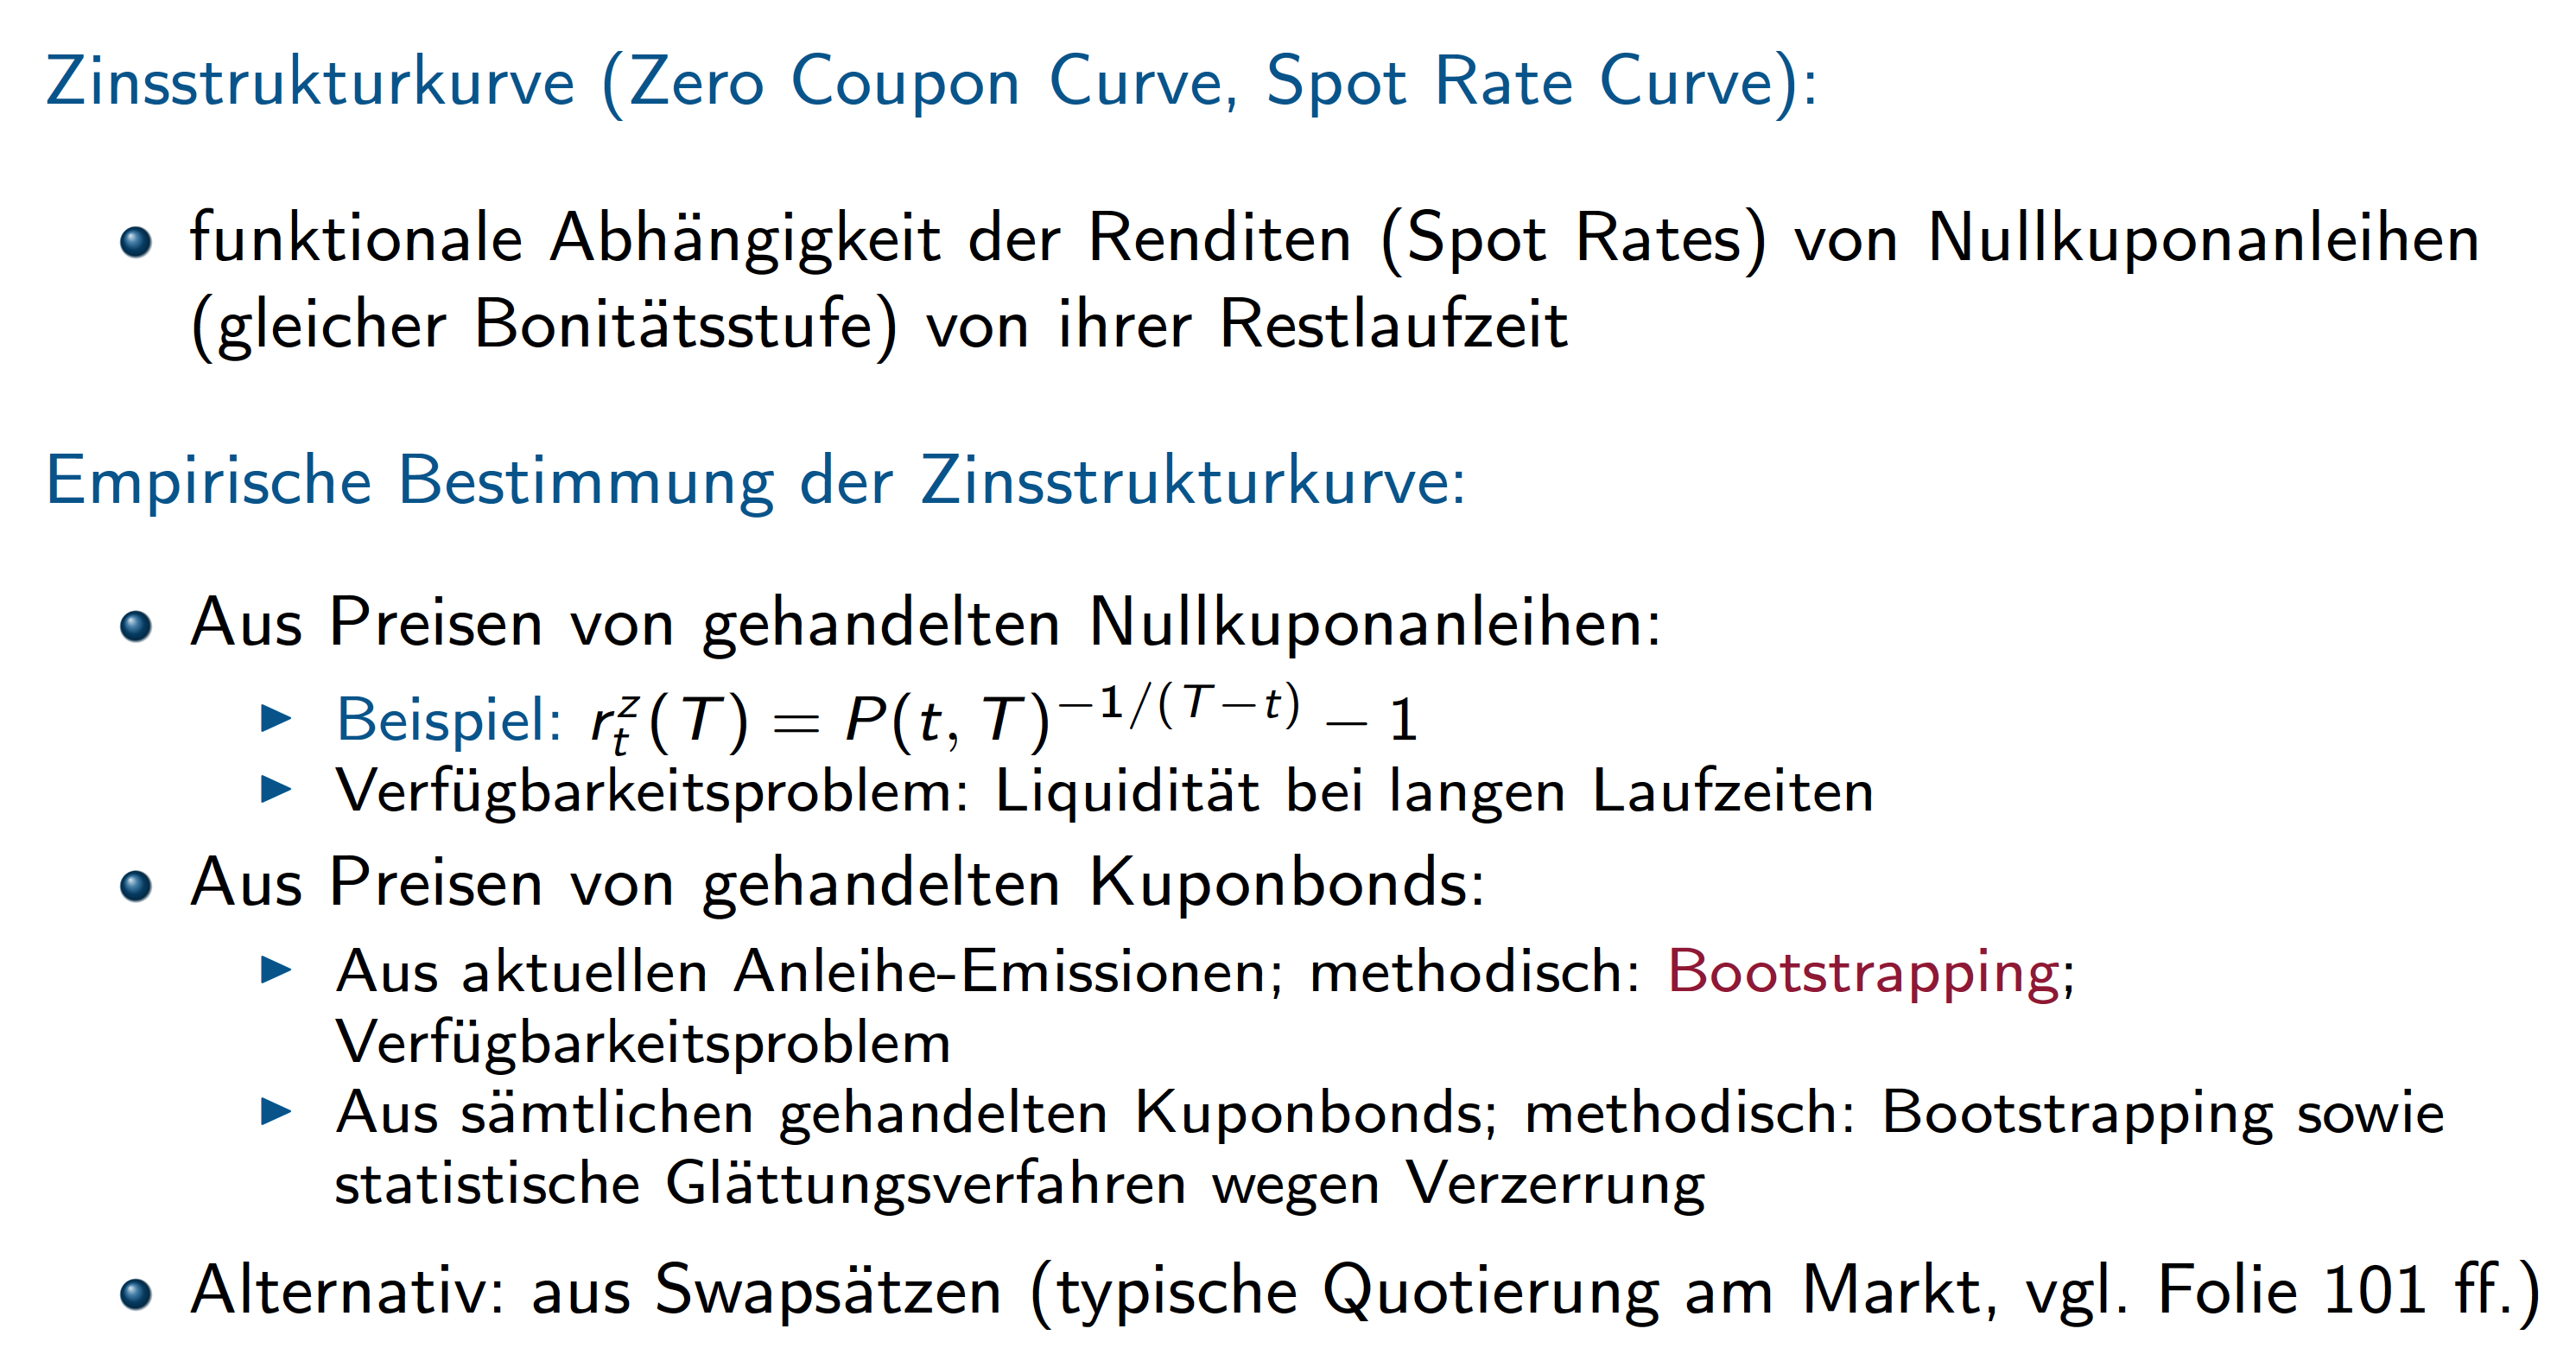
\includegraphics[width=\textwidth]{Bilder/Zinsstrukturkurve.png}
\end{figure}

\subsection{Analyse des Zins\"anderungsrisikos: Duration und Konvexit\"at}

\subsubsection{Annahmen}

\begin{itemize}
	\item Zinsstruktur in $t=0$ flach: $r_0^z (s) = r$ f\"ur alle $s \geq 0$
	\item Zins\"anderung durch einmaligen \"Ubergang in flache Zinsstruktur der H\"ohe $r + \Delta r$
	\item Auswirkungen der Zins\"anderung:
	\begin{itemize}
		\item $\Delta P = P(r + \Delta r) -P(r)$
		\item $\Delta K_T = K_T(r + \Delta r) - K_T(r)$
		\item Steigender Marktzins: Barwert f\"allt, Endwert steigt
		\item Fallender Marktzins: Barwert steigt, Endwert f\"allt
	\end{itemize}
\end{itemize}

\subsubsection{Duration}

\begin{itemize}
	\item Absolute Duration: $DUR^A(r):= -P'(r) = \frac{1}{1+r} \sum_{t=1}^T t Z_t(1+r)^{-t}$
	\item Erste Ableitung der Barwertfunktion mit negativem Vorzeichen
	\item Zins\"anderungsrisiko ist gr\"o{\ss}er, wenn Duration gr\"o{\ss}er
	\item Modifizierte Duration: $DUR^M(r) := \frac{DUR^A}{P(r)} = \frac{P'(r)}{P(r)} = (\frac{1}{1+r}  \sum_{t=1}^T tZ_t(1+r)^{-t}) / P(r)$
	\item Duration von 3 Faktoren beeinflusst:
	\begin{itemize}
		\item Laufzeit der Bonds
		\item H\"ohe des Kupons
		\item Marktzins
	\end{itemize}
	\item d.h.:
	\begin{itemize}
		\item Duration sinkt, wenn Kupon steigt
		\item Duration sinkt, wenn Marktzins steigt
		\item Je l\"anger die Laufzeit, desto gr\"o{\ss}er die Duration
	\end{itemize}
\end{itemize}

\subsection{Komplexere Zinsprodukte}

\subsubsection{\"Uberblick Zinsswap}

\begin{itemize}
	\item Finanzderivat, bei dem zwei Parteien vereinbaren, zu vorher festgesetzten zuk\"unftigen Zeitpunkten Zinszahlungen auf Nennwerte zu tauschen
	\item Vereinfachung: Differenz zwischen Zinszahlungen wird getauscht
	\item Nennwerte stimmen i.d.R. \"uberein
	\item Zins-W\"ahrungs-Swap: Zinsswap auf verschiedenen W\"ahrungen
	\item Typisch: Austausch fester gegen variable Zinsen
	\item Zweck: Absicherung gegen Zins\"anderungen oder Spekulation auf diese
	\item Payer-Swap: Swap aus Sich der Vertragspartei, die den festen Zins zu zahlen hat und daf\"ur den variablen Zinssatz erh\"alt
	\item Receiver-Swap: Swap aus Sich der Vertragspartei, die den variablen Zins zu zahlen hat und daf\"ur den festen Zinssatz erh\"alt
	\item Wert Payer-Swap: $\Pi^p(t) = N(P(t,T_0) - P(t,T_n) - r \delta \sum_{k=1}^n P(t,T_k))$
	\item Wert Receiver-Swap: $\Pi^r(t) = - \Pi^p(t)$ entgegengesetzt zum Payer-Swap
	\item Forward Swap Rate: $\Pi^p(t) = - \Pi^r(t) = 0$
\end{itemize}

\section{Risikoneutrale Bewertung von Aktienderivaten in Binomialb\"aumen}

\subsection{Klassische Aktienderivate}

\begin{itemize}
	\item Aktienderivat: Finanzkontrakt, dessen Auszahlung (Zahlungsstrom) sich aus dem realisierten Kursverlauf einer Aktie ableitet
	\item Formal: $C_t = f(S_0,S_1,...,S_t)$ f\"ur eine Funktion $f$, $(S_t)_{t=0,1,...,T}$ der Aktienpreisprozess, $C_T$ die Auszahlung
	\item Beispiele:
	\begin{itemize}
		\item Call-Option: $C_T^{call} = S_T-K)^+$ mit Aus\"ubungspreis $K>0$
		\item Put-Option: $C_T^{put} = (K-S_T)^+$ mit Aus\"ubungspreis $K>0$
	\end{itemize}
\end{itemize}

\begin{figure}[H]
\centering
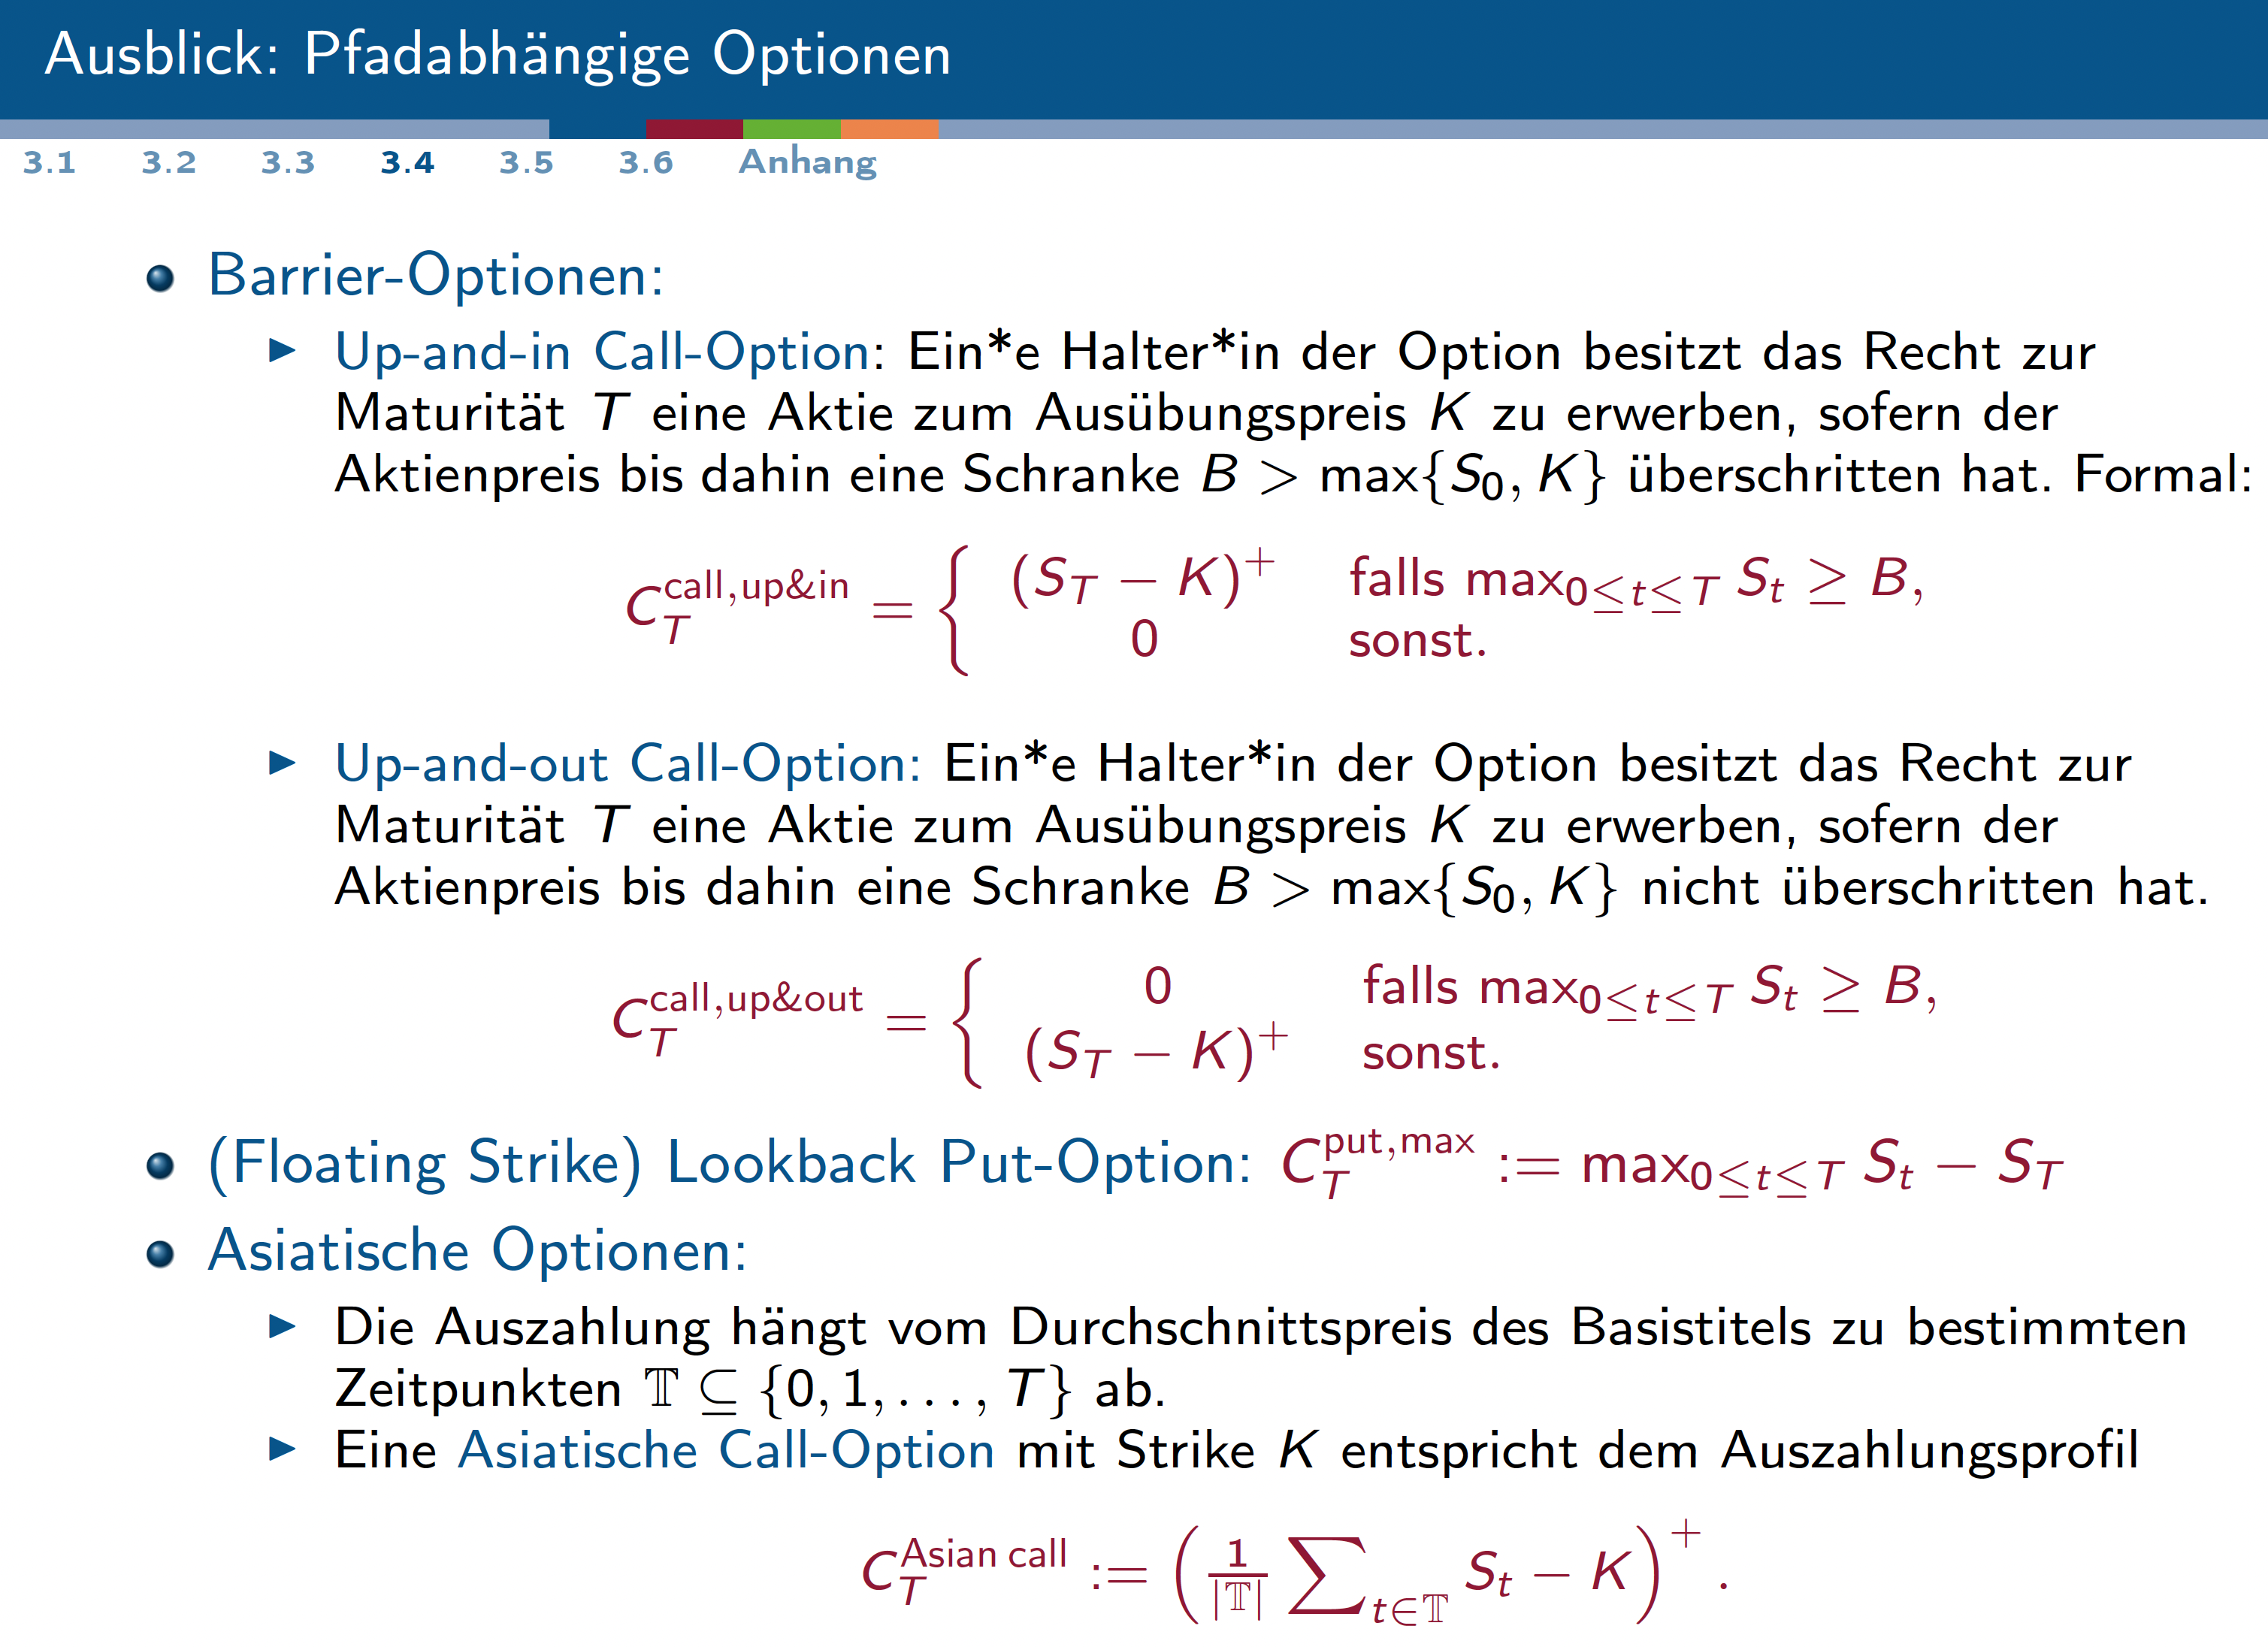
\includegraphics[width=\textwidth]{Bilder/AusblickOptionen.png}
\end{figure}

\subsubsection{Binomialmodell}

\subsubsection{Binomialmarktmodell nach Cox-Ross-Rubinstein}

\begin{itemize}
	\item diskretes Finanzmarktmodell mit $T$ Handelsperioden
	\item Prim\"are Produkte:
	\begin{itemize}
		\item Risikofreie Anlage (Sparbuch): deterministischer Periodenzins $r>-1$, \\ $S_t^0 := (1+r)^t$, $t=0,...,T$
		\item Risikobehaftete Anlage (Aktie): $S:=S^1$
		\begin{itemize}
			\item in jeder Handelsphase Up-Faktor $u$ oder Down-Faktor $d$ unterstellt
			\item Aktienpreis springt entweder auf h\"oheren Wert $S_t = S_{t-1} \cdot u$ oder niedrigeren Wert $S_t = S_{t-1} \cdot d$
		\end{itemize}
	\end{itemize}
\end{itemize}

\begin{figure}[H]
\centering
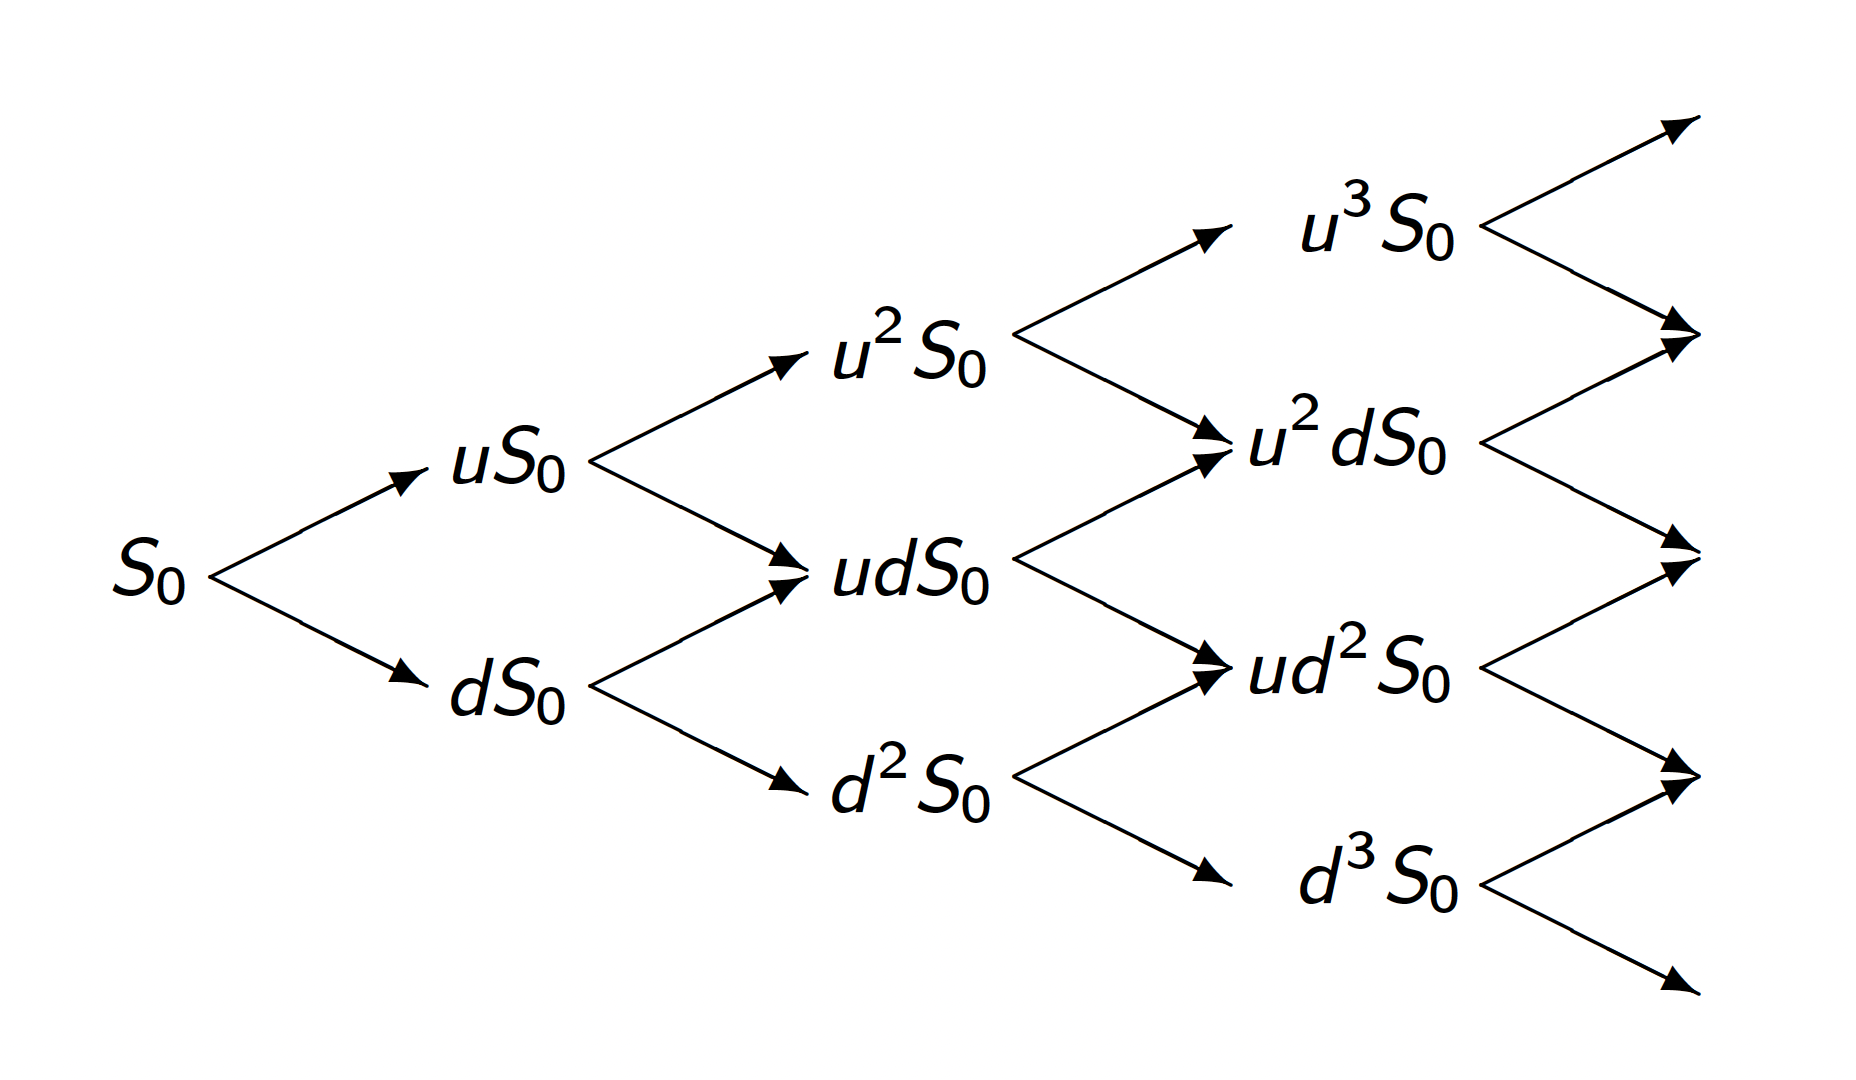
\includegraphics[width=\textwidth]{Bilder/BinomialmodellUpDown.png}
\end{figure}

\begin{figure}[H]
\centering
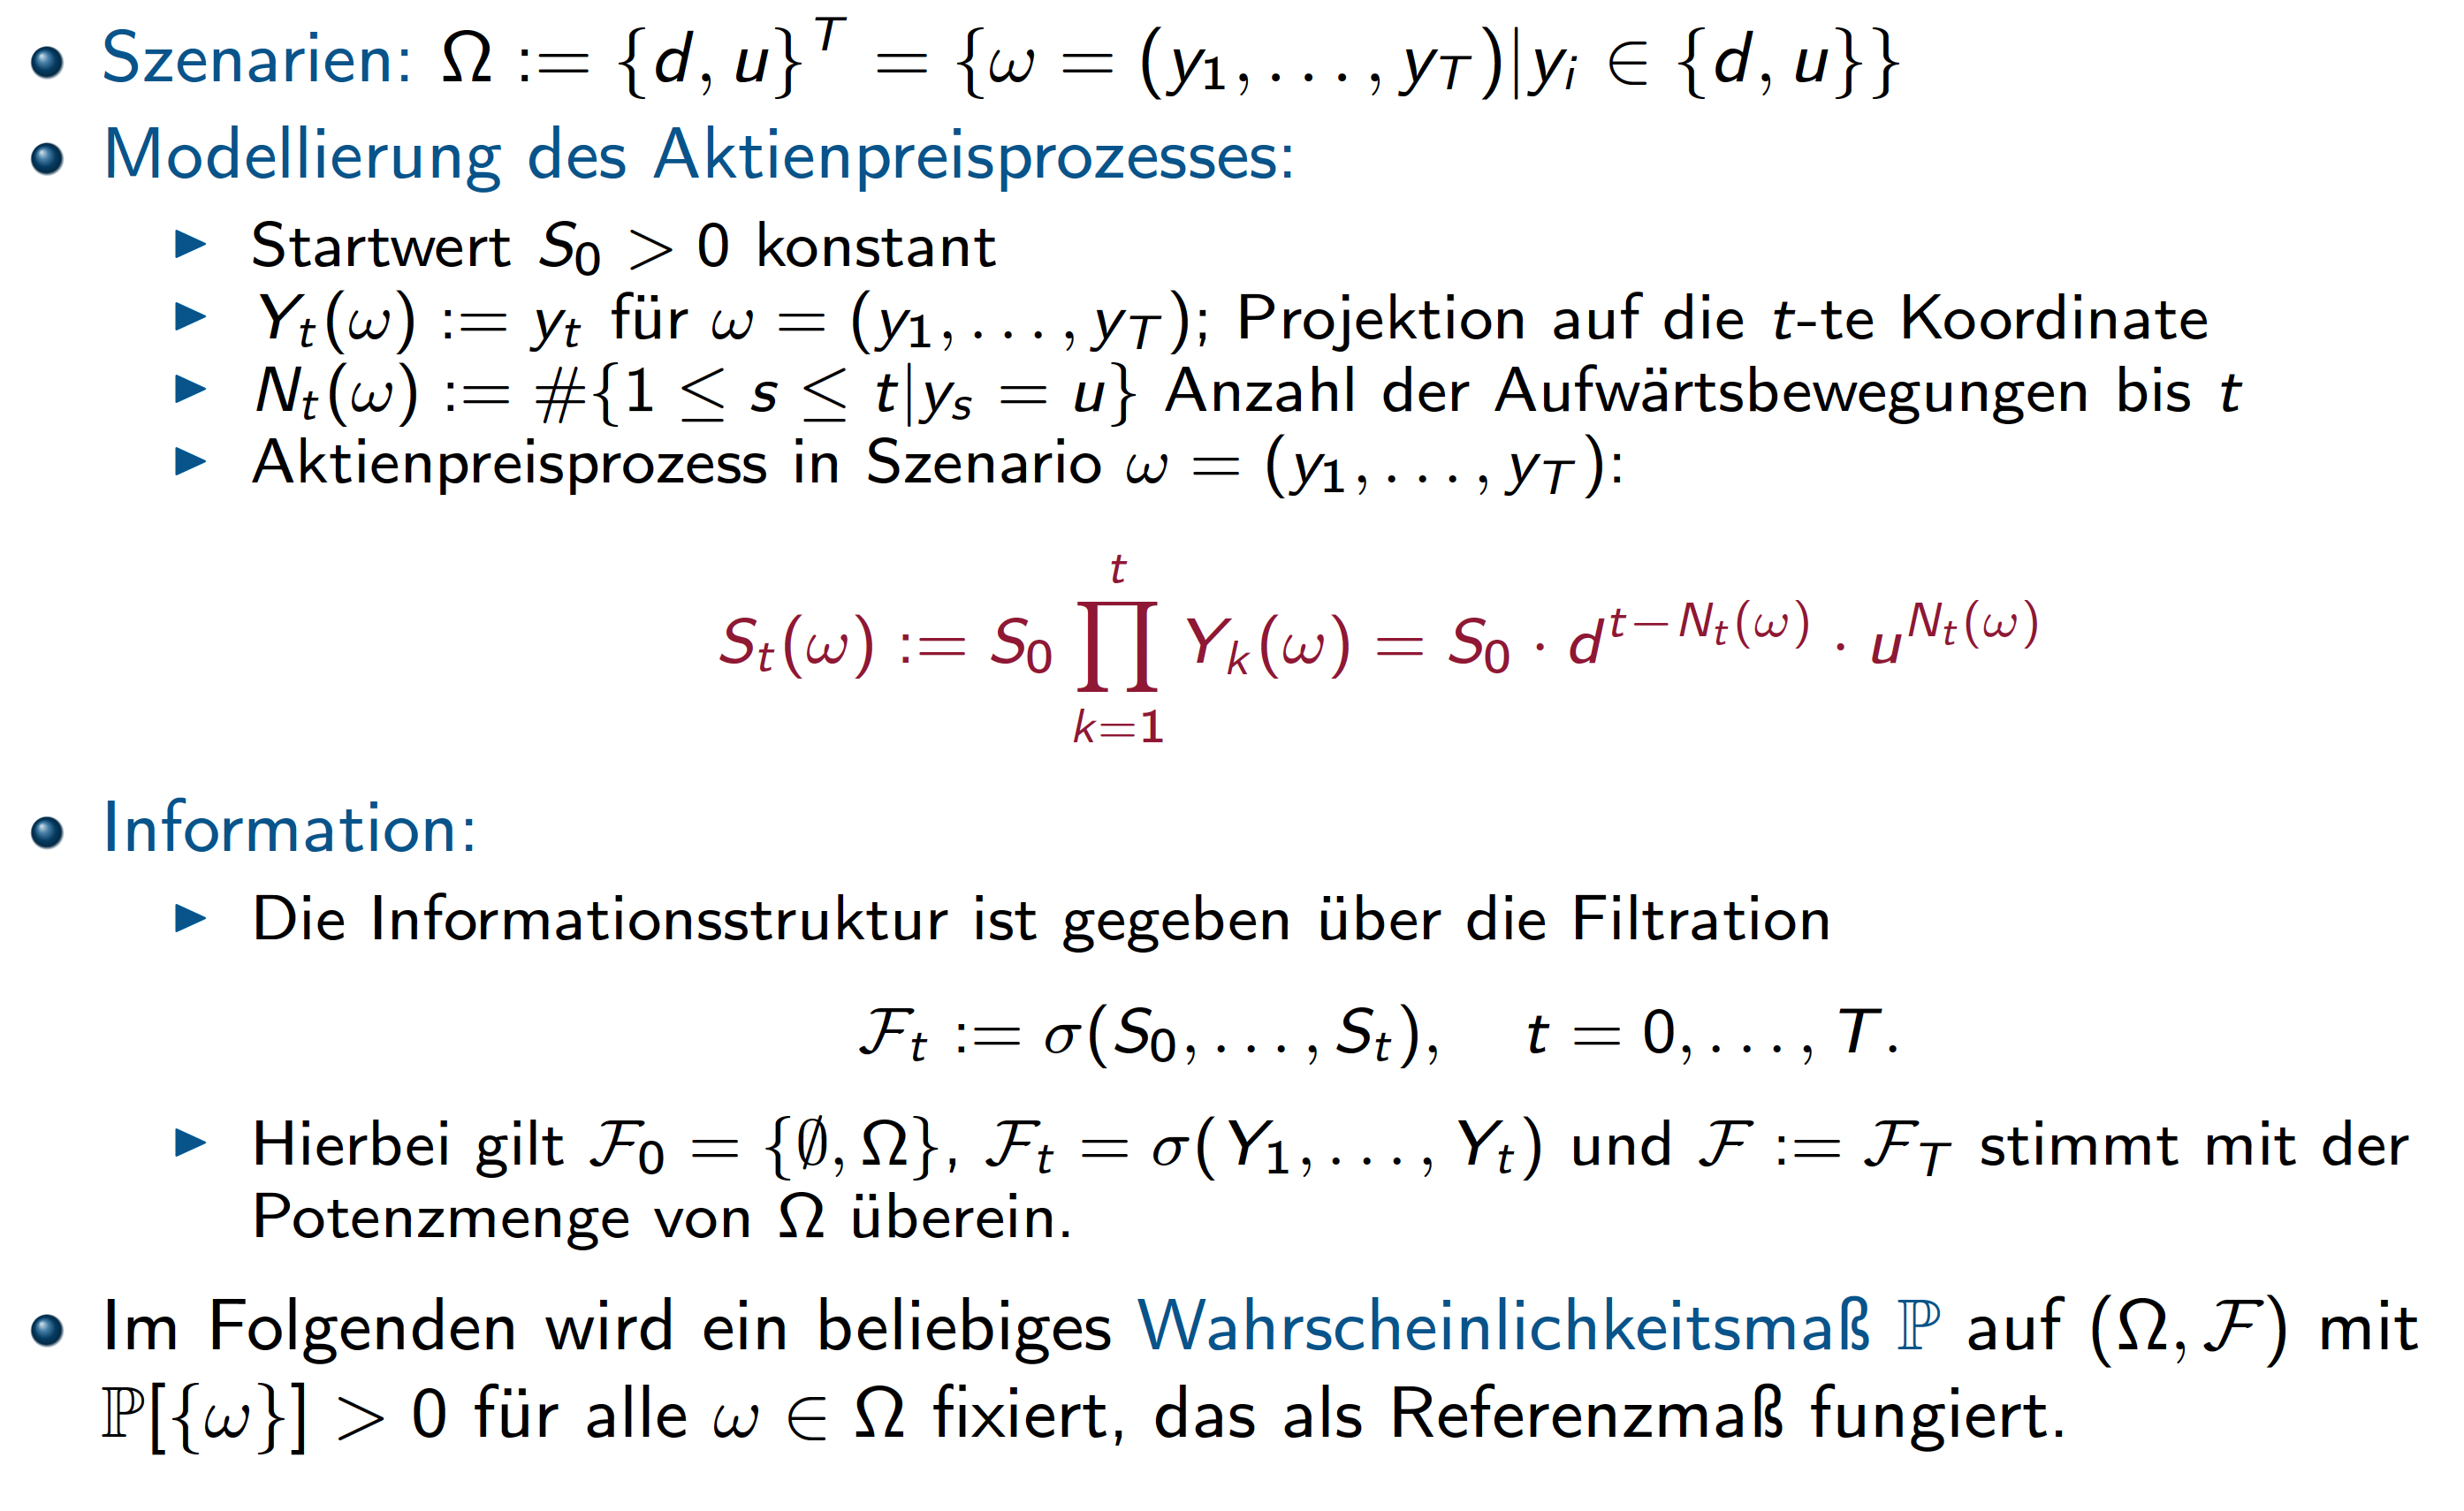
\includegraphics[width=\textwidth]{Bilder/FormaleKonstruktion.png}
\end{figure}

\begin{figure}[H]
\centering
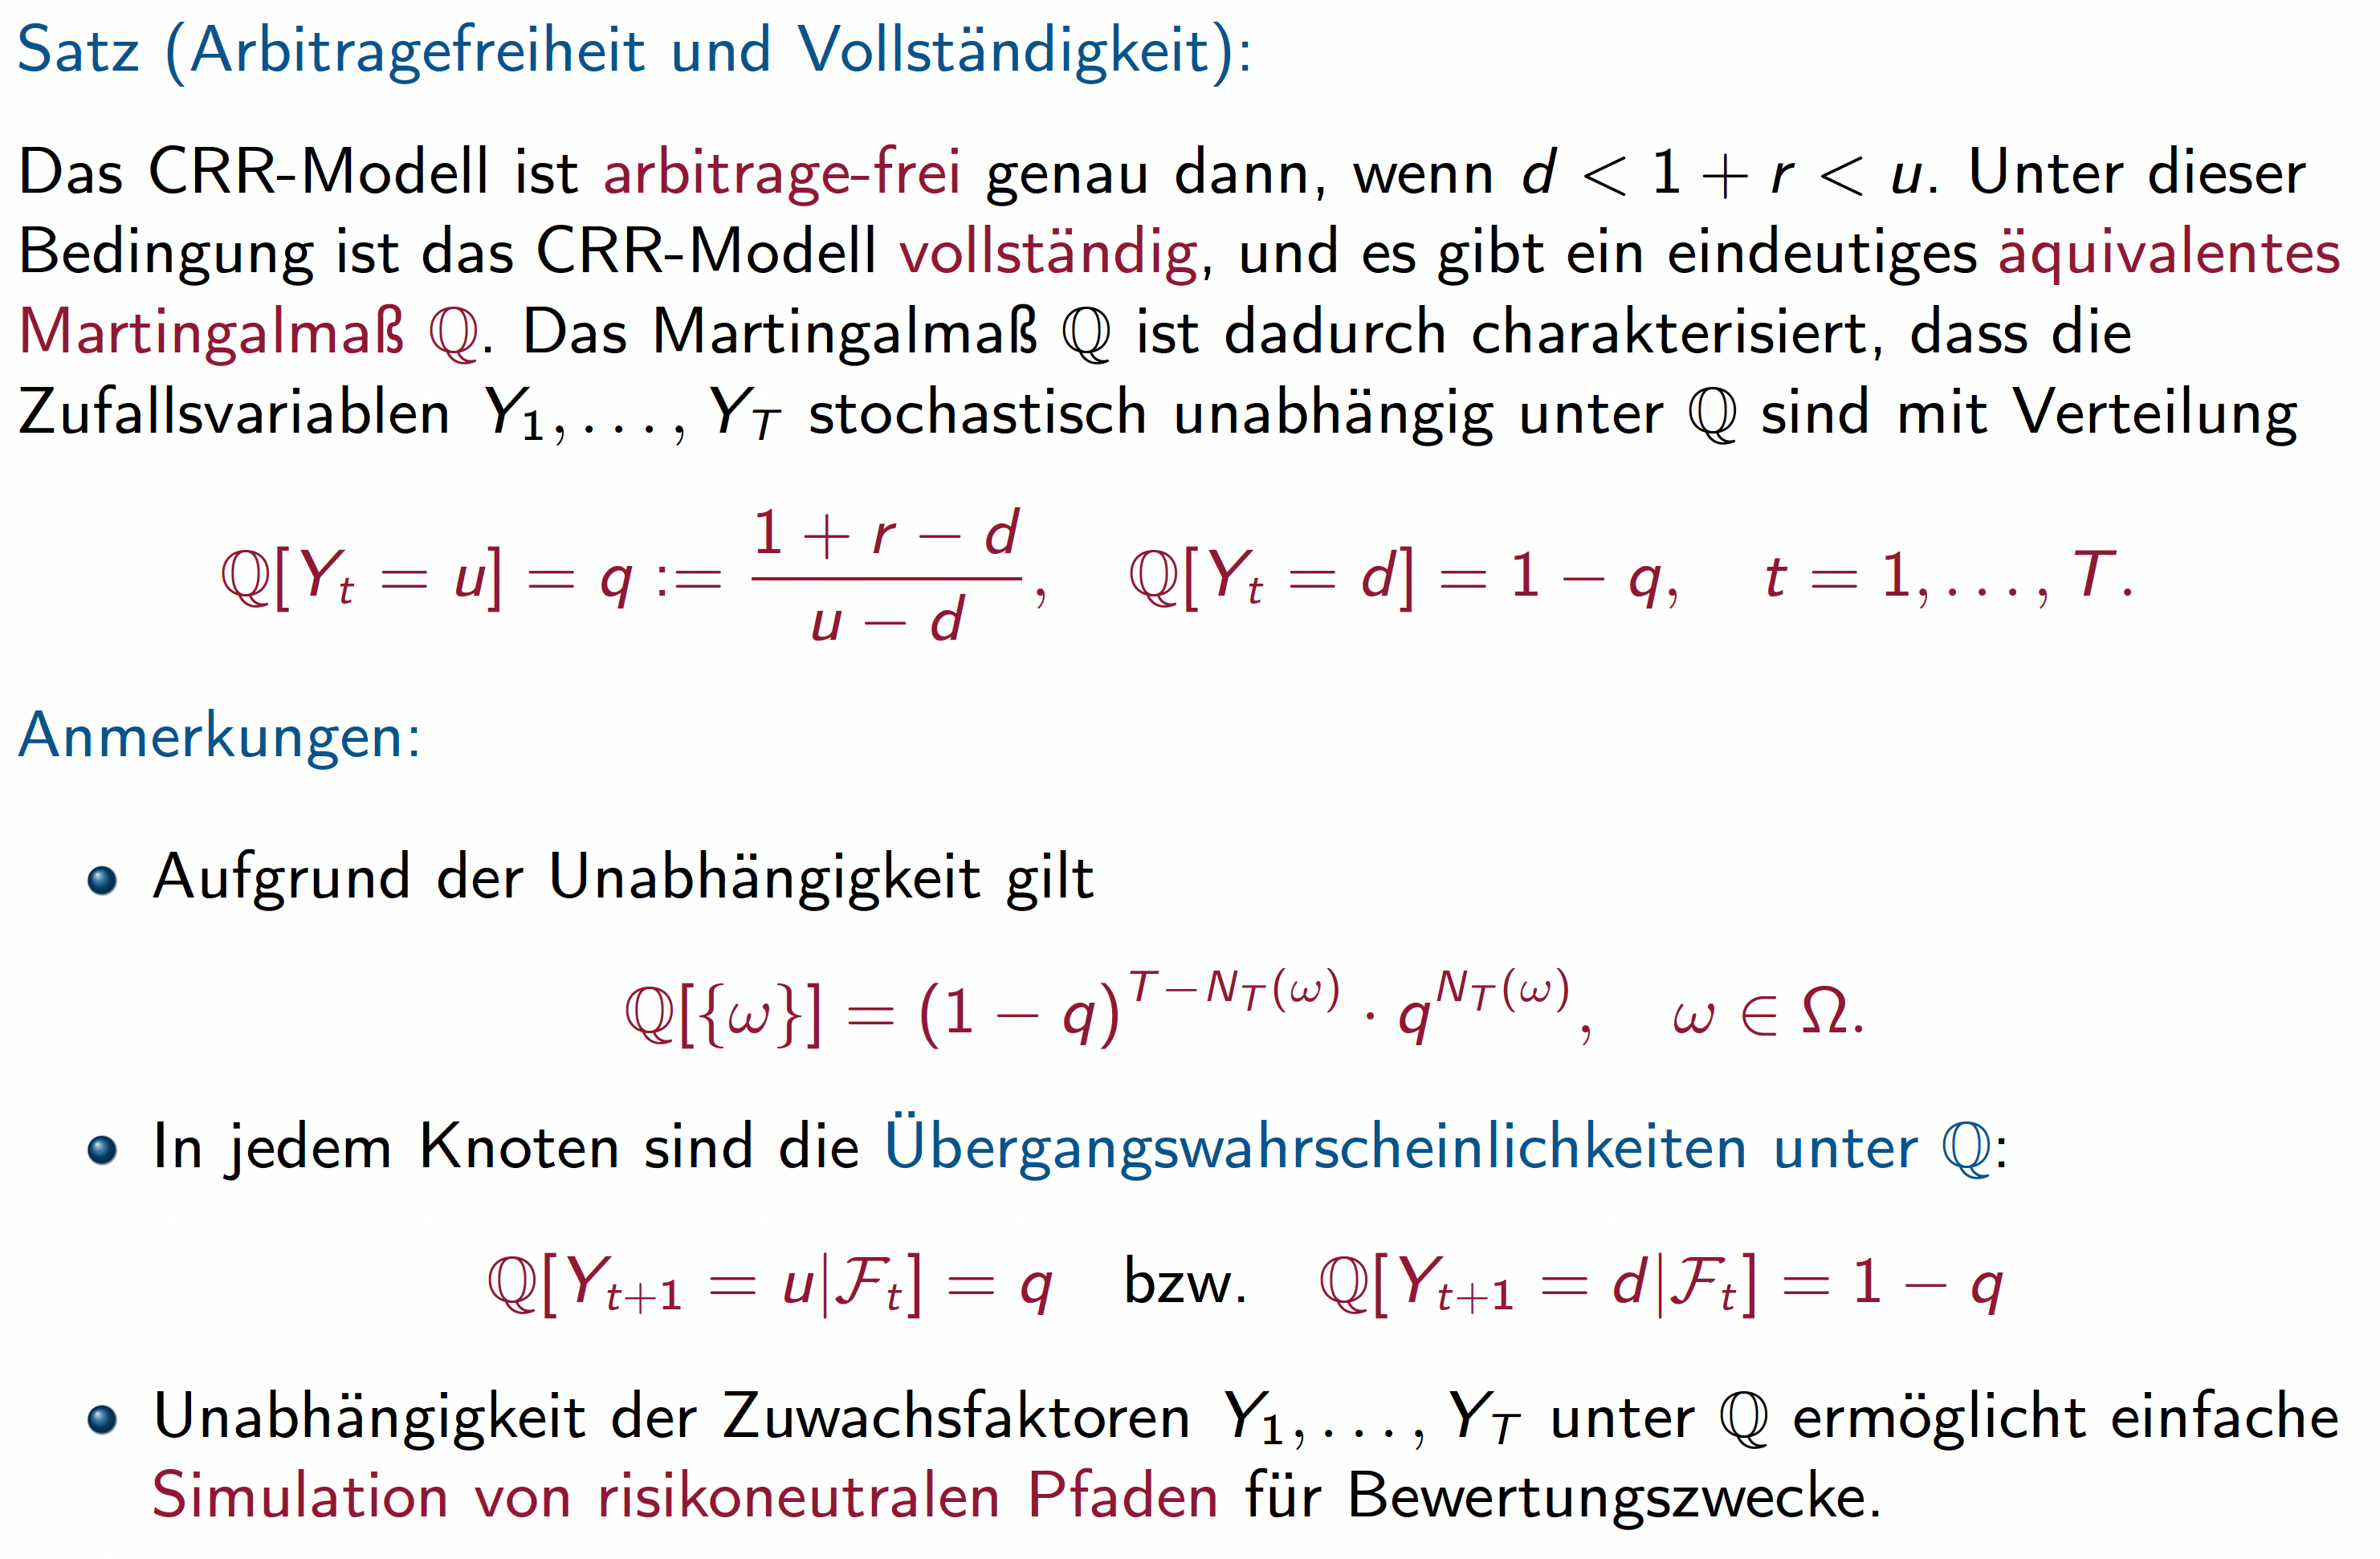
\includegraphics[width=\textwidth]{Bilder/SatzArbitragefreiheit.png}
\end{figure}

\section{Vom Binomialmodell zum Black-Scholes-Modell}

\subsection{Konvergenz gegen den Black-Scholes-Preis}

?



























\end{document}
